% !TEX program = xelatex
% =====================================================================
%  guide.tex  --  user guide for the mynotes notes & slides template
%  Every "demo" box shows the LaTeX source on top and the result below.
% =====================================================================
\documentclass[11pt]{article}
\usepackage{mynotes}
\notesetup{User Guide}{Author Name}{https://example.com}

% ---- only for this guide: a box that shows source + result ----
\lstdefinestyle{latexsrc}{style=notes, language=[LaTeX]TeX,
  texcsstyle=*\color{code-kw}, moretexcs={notesetup,notetitle,hl,code,cref,Cref,vect,R,
  pyfile,thead,newcallout,includegraphics,captionof,addplot,State,Function,Return,
  EndFunction,For,EndFor,If,EndIf,Require,Ensure,Repeat,Until,toprule,midrule,bottomrule,
  rowcolor,multirow,norm,abs,inner,spn,rank,tr,showsolutionsfalse,usetheme,website,
  titleframe,closingframe,sectionframe,institute,subtitle,definecolor,eqref}}
% Source box (gray, "LaTeX") followed by the rendered result, marked by a rule.
\makeatletter
\tcbset{demosrc/.style={enhanced, breakable, listing only,
  colback=codebg, colframe=codeframe, boxrule=0.5pt, arc=2pt,
  left=6pt, right=6pt, top=2pt, bottom=2pt, before skip=6pt, after skip=4pt,
  listing options={style=latexsrc},
  fonttitle=\ttfamily\small\bfseries, coltitle=bodytext!80,
  colbacktitle=codeframe!45, titlerule=0pt, toptitle=1pt, bottomtitle=1pt,
  title={\nb@icon{F121}\enspace LaTeX source \hfill result below\enspace\nb@icon{F063}}}}
% (reset: boxes inside the result must not inherit the source box's title & colors)
\newcommand{\demoresult}{\par\vspace{2pt}%
  \begingroup\tcbset{reset}\input{\jobname.listing}\endgroup\par\nobreak\vspace{2pt}%
  {\color{codeframe}\noindent\rule{\linewidth}{0.8pt}}\par\vspace{4pt}}
\newtcblisting{demosource}{demosrc, title={\nb@icon{F121}\enspace LaTeX source}}  % source only
\makeatother
\newtcblisting{demo}{demosrc, after app={\demoresult}}  % source + result

\begin{document}
\notetitle{Notes \& Slides Template: User Guide}

\begin{tldr}
One style for \textbf{lecture notes}, \textbf{books of notes} and \textbf{Beamer
slides}: colored theorem boxes, Obsidian-style callouts, syntax-highlighted code,
striped tables and plots, all in IBM Plex Mono. Compile with \textbf{XeLaTeX} (or
LuaLaTeX). In this guide, each gray \textbf{LaTeX source} box is followed by its
\textbf{result}, closed by a gray rule. Copy what you need.
\end{tldr}

\tableofcontents

% =====================================================================
\section{Quick start}\label{sec:start}

\subsection{On Overleaf}

\begin{enumerate}
  \item Open the template and click \textbf{Open as Template} (or upload the
        project as a \code{.zip} via \textbf{New Project} $\to$ \textbf{Upload Project}).
  \item Open \textbf{Menu} $\to$ \textbf{Compiler} and choose \textbf{XeLaTeX}.
        (The included \code{latexmkrc} does this too.)
  \item In \textbf{Menu} $\to$ \textbf{Main document}, pick the file you want to
        build: \code{note.tex}, \code{main.tex}, \code{slides.tex} or \code{guide.tex}.
  \item Click \textbf{Recompile}.
\end{enumerate}

\subsection{On your computer}

You need a recent TeX distribution (TeX Live, MacTeX or MiKTeX) with XeLaTeX and
\code{latexmk}. From the template folder:

\begin{terminal}[Terminal]
$ latexmk note.tex          # one document
$ latexmk                   # every document listed in latexmkrc
$ latexmk -c                # remove auxiliary files
\end{terminal}

\begin{tip}[VS Code with LaTeX Workshop]
Every main file starts with \code{\% !TEX program = xelatex}. LaTeX Workshop reads
this line and uses XeLaTeX automatically. Keep it as the first line of every new
main file.
\end{tip}

\begin{warning}
pdfLaTeX is \emph{not} supported: the template uses system fonts through
\code{fontspec}. If you compile with pdfLaTeX you get a clear error message
asking you to switch.
\end{warning}

% =====================================================================
\needspace{12\baselineskip}   % keep the heading together with the table below
\section{What is in the template}

\begin{widetable}[Files in the template][tab:files]{lL}
\thead{File / folder} & \thead{Purpose} \\
\midrule
\code{note.tex}    & Start here for a \textbf{single-topic note} (one file per topic). \\
\code{main.tex}    & Start here for a \textbf{book of notes} (chapters, table of contents). \\
\code{slides.tex}  & Start here for a \textbf{talk} (Beamer, 16:9). \\
\code{guide.tex}   & This user guide. \\
\code{mynotes.sty} & Layout of the notes: page, headings, header and footer. \\
\code{beamerthememynotes.sty} & Layout of the slides: Beamer theme. \\
\code{mynotes-core.sty} & Shared by both: fonts, colors, boxes, callouts, code, tables, figures, macros. \\
\code{chapters/}   & Sample content used by \code{note.tex} and \code{main.tex}. Replace it with your own files. \\
\code{code/}       & Example source file shown with \code{\pyfile}. \\
\code{fonts/}      & IBM Plex Mono and Font Awesome. Must sit next to your main \code{.tex} file. \\
\code{latexmkrc}   & Build settings (XeLaTeX) for \code{latexmk} and Overleaf.
\end{widetable}

\subsection{A single note}

\begin{demosource}
% !TEX program = xelatex
\documentclass[11pt]{article}
\usepackage{mynotes}
\notesetup{Short Title}{Author Name}{https://example.com}  % header & footer

\begin{document}
\notetitle{Full Title of the Note}   % big title + author | date
\section{Introduction}
...
\end{document}
\end{demosource}

\code{\notesetup} takes three arguments: the short title (left of the header), the
author (left of the footer) and a website the author name links to. Leave the
website empty, \code{\notesetup{Title}{Author Name}{}}, for no link.

\subsection{A book of notes}

Use the \code{book} class and put one chapter per file in \code{chapters/}. Each
chapter starts on a new page; the header shows the current chapter.

\begin{demosource}
% !TEX program = xelatex
\documentclass[11pt,oneside]{book}
\usepackage{mynotes}
\notesetup{Course Name}{Author Name}{https://example.com}
% \showsolutionsfalse     % hide all solutions (student handout)

\begin{document}
\tableofcontents
\chapter{First Chapter}
% ---------------------------------------------------------------------
%  Sample content: text, lists and mathematics
% ---------------------------------------------------------------------
\section{Text and lists}\label{sec:text}

This document is a sample built with the template. Each section shows one
kind of element, so you can see the final look before writing your own notes.
Replace this text with your content.

Body text supports \emph{emphasis}, \textbf{bold text},
\hl{highlighted key terms}, inline code such as \code{result = compute(data)},
and links such as \href{https://example.com}{example.com}.\footnote{Footnotes
appear at the bottom of the page.}

\begin{itemize}
  \item Bullet lists use the accent color.
  \item They can be nested:
  \begin{itemize}
    \item a second-level item
    \item another second-level item
  \end{itemize}
  \item[\textcolor{co-green}{\checkmark}] Custom markers are possible too.
\end{itemize}

\begin{enumerate}
  \item Numbered lists
  \item keep the spacing compact
  \item and align neatly.
\end{enumerate}

\subsection{A subsection}

Subsections and subsubsections share the accent color, with smaller sizes.
The header of each page shows the current section.

\subsubsection{A subsubsection}

Paragraphs are separated by a small gap instead of an indent, which keeps
notes easy to scan.

% ---------------------------------------------------------------------
\section{Mathematics}\label{sec:math}

Inline math sits in the text: $f\colon \R^n \to \R$, $\norm{\vect{x}}$,
$\abs{a - b}$ and $\inner{\vect{u}}{\vect{v}}$. Letters and digits use the same
typeface as the text.

A numbered equation can be referenced later:
\begin{equation}\label{eq:sample}
  \int_a^b f(x)\,dx = F(b) - F(a).
\end{equation}

A multi-line derivation, aligned at the equals sign, with only the last line
numbered:
\begin{align}
  (a + b)^2 &= (a + b)(a + b) \nonumber\\
            &= a^2 + 2ab + b^2. \label{eq:aligned}
\end{align}

Matrices, sums, fractions and cases:
\[
  A = \begin{bmatrix} a_{11} & a_{12} \\ a_{21} & a_{22} \end{bmatrix},
  \qquad
  \sum_{k=1}^{n} k = \frac{n(n+1)}{2},
  \qquad
  \abs{x} = \begin{cases} x, & x \ge 0, \\ -x, & x < 0. \end{cases}
\]
References such as \eqref{eq:sample} and \eqref{eq:aligned} are clickable links.

% ---------------------------------------------------------------------
%  Sample content: numbered boxes
% ---------------------------------------------------------------------
\section{Numbered boxes}\label{sec:boxes}

Numbered boxes hold the content you will refer back to. Each one takes an
optional title and an optional label; the number follows the section.

\begin{definition}[Title of the definition][def:sample]
A \emph{definition} states precisely what a term means. For example, a
function $f$ is \emph{increasing} if $x < y$ implies $f(x) \le f(y)$.
\end{definition}

\begin{theorem}[Title of the theorem][thm:sample]
A \emph{theorem} states a main result. If $f$ and $g$ are increasing, then
$f + g$ is increasing.
\end{theorem}

\begin{proof}
Let $x < y$. By \cref{def:sample}, $f(x) \le f(y)$ and $g(x) \le g(y)$.
Adding the two inequalities gives $(f + g)(x) \le (f + g)(y)$.
\end{proof}

\begin{lemma}
Lemmas, propositions and corollaries share the color and the counter of
theorems.
\end{lemma}

\begin{corollary}
By \cref{thm:sample}, any finite sum of increasing functions is increasing.
\end{corollary}

\begin{example}[][ex:sample]
Examples are shown in blue. Both $f(x) = x$ and $g(x) = x^3$ are increasing,
so $x + x^3$ is increasing as well.
\end{example}

\begin{remark}
Remarks are gray, for side comments that do not need emphasis.
\end{remark}

\begin{exercise}[][exer:sample]
Exercises are orange. Show that $h(x) = -x$ is not increasing.
\end{exercise}

\begin{solution}
Take $x = 0 < 1 = y$. Then $h(0) = 0 > -1 = h(1)$. Solutions can be hidden
for handouts with \code{\showsolutionsfalse}.
\end{solution}

   % starts with \chapter{...}
\chapter{Second Chapter}
% ---------------------------------------------------------------------
%  Sample content: callouts
% ---------------------------------------------------------------------
\section{Callouts}\label{sec:callouts}

Callouts are unnumbered side notes. Each type has its own color and icon, and
any of them accepts a custom title in brackets.

\begin{note}
Use a note for extra context the reader may find useful.
\end{note}

\begin{info}
Use info for background information or a quick fact.
\end{info}

\begin{tip}[A custom title]
This tip has a custom title instead of the default one.
\end{tip}

\begin{important}
Use important for something the reader should not skip.
\end{important}

\begin{summary}
Use a summary to wrap up a section in one or two sentences.
\end{summary}

\begin{success}
Use success for a confirmed result or a check that passed.
\end{success}

\begin{question}
Use a question to make the reader think before reading on.
\end{question}

\begin{warning}
Use a warning for a common mistake or a condition that must hold.
\end{warning}

\begin{failure}
Use failure for an approach that does not work, and why.
\end{failure}

\begin{danger}
Use danger for a step that can cause serious errors.
\end{danger}

\begin{bug}
Use bug for a known issue or a correction.
\end{bug}

\begin{todo}
Use todo for a reminder of work still to be done.
\end{todo}

\begin{quotebox}[Author of the quote]
A quotation, with its source as the title.
\end{quotebox}

The types \code{hint}, \code{tldr}, \code{faq}, \code{caution} and
\code{attention} are also available, and new ones can be defined with
\code{\newcallout}.

% ---------------------------------------------------------------------
%  Sample content: code, tables, figures and algorithms
% ---------------------------------------------------------------------
\section{Code}\label{sec:code}

A whole source file, with line numbers and the file name as the title:

\pyfile{code/example.py}

Program output in a terminal block:

\begin{terminal}
$ python code/example.py
mean = 5.00, std = 2.00
\end{terminal}

Any language supported by the \code{listings} package:

\begin{codeblock}{C++}[main.cpp]
#include <iostream>

int main() {
    std::cout << "Hello, world!" << std::endl;
    return 0;
}
\end{codeblock}

% ---------------------------------------------------------------------
\section{Tables and figures}\label{sec:tables}

Tables and figures stay exactly where they are written. The first row of a
table is the header; the rows below it are striped automatically.

\begin{datatable}[A striped table][tab:sample]{lccr}
\thead{Item} & \thead{Group} & \thead{Status} & \thead{Value} \\
\midrule
Alpha & A & done & 12.5 \\
Beta  & A & open &  8.0 \\
Gamma & B & done & 15.2 \\
Delta & B & open &  4.7
\end{datatable}

\begin{widetable}[A full-width table with wrapping text][tab:wide]{lLl}
\thead{Element} & \thead{Description} & \thead{Example} \\
\midrule
Box     & Numbered content with an optional title and a label for references. & \code{theorem} \\
Callout & Unnumbered side note with an icon, in one of six colors.            & \code{warning} \\
Code    & Highlighted source code with line numbers and a file name.          & \code{python}
\end{widetable}

\begin{notefigure}[A plot drawn with pgfplots][fig:plot]
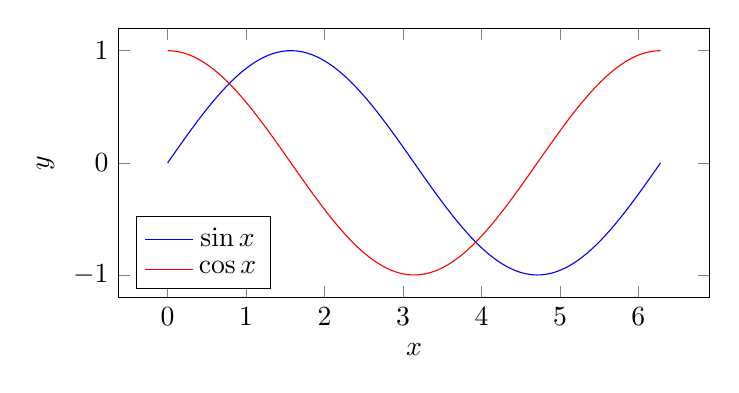
\begin{tikzpicture}
\begin{axis}[width=0.75\linewidth, height=5cm, xlabel={$x$}, ylabel={$y$},
             domain=0:6.283, samples=100, legend pos=south west]
  \addplot+[no marks] {sin(deg(x))};
  \addplot+[no marks] {cos(deg(x))};
  \legend{$\sin x$, $\cos x$}
\end{axis}
\end{tikzpicture}
\end{notefigure}

\begin{notefigure}[Images from files, side by side][fig:images]
  \begin{subfigure}{0.32\linewidth}\centering
    \includegraphics[width=\linewidth]{example-image-a}\caption{First image}
  \end{subfigure}\quad
  \begin{subfigure}{0.32\linewidth}\centering
    \includegraphics[width=\linewidth]{example-image-b}\caption{Second image}
  \end{subfigure}
\end{notefigure}

% ---------------------------------------------------------------------
\section{Algorithms}\label{sec:algorithms}

\begin{algorithm}[H]
\caption{A generic iterative procedure}\label{alg:sample}
\begin{algorithmic}[1]
\Require input data $D$, tolerance $\varepsilon > 0$
\Ensure result $r$
\State $r \gets$ initial guess
\Repeat
  \For{each item $d \in D$}
    \State update $r$ using $d$
  \EndFor
\Until{the change in $r$ is smaller than $\varepsilon$}
\State \Return $r$
\end{algorithmic}
\end{algorithm}

% ---------------------------------------------------------------------
\section{Cross-references}\label{sec:refs}

Every labeled element can be referenced by name and number, and each
reference is a link: \cref{def:sample}, \cref{thm:sample}, \cref{ex:sample},
\cref{eq:sample}, \cref{tab:sample}, \cref{fig:plot}, \cref{alg:sample} and
\cref{sec:math}.

\begin{summary}
One style for notes, books and slides. Replace the sample content with your
own and keep the structure.
\end{summary}


\end{document}
\end{demosource}

% =====================================================================
\section{Text, lists and links}

\begin{demo}
Use \emph{emphasis}, \textbf{bold}, \hl{highlighted terms},
inline code like \code{compute(x)}, and links:
\href{https://example.com}{a website}.

\begin{itemize}
  \item bullet points
  \item[\textcolor{co-green}{\checkmark}] custom bullet
\end{itemize}
\begin{enumerate}
  \item numbered
  \item lists\footnote{Footnotes work too.}
\end{enumerate}
\end{demo}

% =====================================================================
\section{Math}

\begin{demo}
Inline: $\vect{x} \in \R^n$, $\norm{\vect{x}}$, $\inner{\vect{x}}{\vect{y}}$.
Numbered equation:
\begin{equation}\label{eq:sample}
  \int_a^b f(x)\,dx = F(b) - F(a)
\end{equation}
Aligned steps, only the last one numbered:
\begin{align}
  (a + b)^2 &= (a + b)(a + b) \nonumber\\
            &= a^2 + 2ab + b^2 \label{eq:aligned}
\end{align}
Matrices: $A = \begin{bmatrix} 0 & 1 \\ 0 & 0 \end{bmatrix}$.
\end{demo}

\begin{datatable}[Math shortcuts defined by the template][tab:macros]{ll}
\thead{Command} & \thead{Result} \\
\midrule
\code{\R \N \Z \Q \C} & $\R\ \N\ \Z\ \Q\ \C$ \\
\code{\vect{x}} & $\vect{x}$ \\
\code{\abs{x}}, \code{\norm{x}}, \code{\inner{x}{y}} & $\abs{x}$, $\norm{x}$, $\inner{x}{y}$ \\
\code{\spn}, \code{\rank}, \code{\tr} & $\spn$, $\rank$, $\tr$
\end{datatable}

\begin{note}
Letters and digits in math use IBM Plex Mono so they match the text; symbols,
operators and Greek come from Latin Modern Math. For classic all-Latin-Modern math,
load \code{\usepackage[classicmath]{mynotes}} (or \code{\usetheme[classicmath]{mynotes}}
in slides).
\end{note}

% =====================================================================
\section{Numbered boxes}

Every box takes an optional \textbf{title} and an optional \textbf{label}, in
that order, and both can be left out:

\begin{demosource}
\begin{theorem}[Title][thm:key] ... \end{theorem}
\end{demosource}

Available: \code{definition}, \code{example}, \code{theorem}, \code{lemma},
\code{proposition}, \code{corollary}, \code{exercise} and \code{remark}, plus
\code{proof} and \code{solution}. Lemmas, propositions and corollaries share
the theorem counter.

\begin{demo}
\begin{definition}[Increasing function][def:inc]
$f$ is increasing if $x < y$ implies $f(x) \le f(y)$.
\end{definition}

\begin{theorem}[Sum of increasing functions][thm:sum]
If $f$ and $g$ are increasing, then so is $f + g$.
\end{theorem}
\begin{proof}
Add $f(x) \le f(y)$ and $g(x) \le g(y)$ (\cref{def:inc}).
\end{proof}

\begin{example}
$f(x) = x$ and $g(x) = x^3$ are increasing, so $x + x^3$ is too.
\end{example}

\begin{exercise}
Show that $h(x) = -x$ is not increasing.
\end{exercise}
\begin{solution}
$0 < 1$, but $h(0) = 0 > -1 = h(1)$.
\end{solution}
\end{demo}

\begin{tip}[Student handouts]
Put \code{\showsolutionsfalse} in the preamble to hide every \code{solution}.
Exercises stay; only the solutions disappear.
\end{tip}

% =====================================================================
\section{Callouts}

Callouts are unnumbered side remarks in the style of Obsidian. Each has a default
title, which you can replace in brackets.

\begin{demo}
\begin{warning}
Check the assumptions before applying a theorem.
\end{warning}
\begin{question}[A custom title]
Any callout accepts a custom title in brackets.
\end{question}
\end{demo}

\begin{datatable}[All callout types][tab:callouts]{ll}
\thead{Color} & \thead{Environments} \\
\midrule
Blue   & \code{note}, \code{info}, \code{todo} \\
Teal   & \code{tip}, \code{hint}, \code{important}, \code{summary}, \code{tldr} \\
Green  & \code{success} \\
Orange & \code{question}, \code{faq}, \code{warning}, \code{caution}, \code{attention} \\
Red    & \code{failure}, \code{danger}, \code{bug} \\
Gray   & \code{quotebox}
\end{datatable}

Define your own callout type in the preamble. The icon is the hexadecimal code
shown for each icon on \href{https://fontawesome.com/icons}{fontawesome.com}
(free, solid style):

\begin{demosource}
% \newcallout{name}{color}{icon}{default title}
\newcallout{idea}{co-orange}{F0EB}{Idea}   % then: \begin{idea} ... \end{idea}
\end{demosource}

% =====================================================================
\section{Tables}

Tables are placed exactly where you write them; they never float to another
page. The first row is the header; the rows after it are striped automatically.

\begin{demo}
\begin{datatable}[A striped table][tab:sample]{lccr}
\thead{Item} & \thead{Group} & \thead{Status} & \thead{Value} \\
\midrule
Alpha & A & done & 12.5 \\
Beta  & A & open &  8.0 \\
Gamma & B & done & 15.2
\end{datatable}
\Cref{tab:sample} shows the default table style.
\end{demo}

For long text, \code{widetable} spans the full width. Use \code{L} (left) or
\code{C} (centered) for columns that should wrap:

\begin{demo}
\begin{widetable}[Document types][tab:types]{lLl}
\thead{Type} & \thead{Description} & \thead{Class} \\
\midrule
Note  & A single topic in one file, with sections.   & article \\
Book  & Several chapters with a table of contents.   & book \\
Talk  & Slides with the same boxes and callouts.     & beamer
\end{widetable}
\end{demo}

% =====================================================================
\section{Code}

\subsection{Python blocks}

\begin{demo}
\begin{python}[greet.py]
def greet(name):
    # Return a short greeting
    return f"Hello, {name}!"

for name in ["Ada", "Alan"]:
    print(greet(name))
\end{python}
\end{demo}

Leave out the title for a plain block: \code{\begin{python} ... \end{python}}.

\subsection{Include a whole file}\label{sec:pyfile}

\begin{demo}
\pyfile{code/example.py}
\end{demo}

\subsection{Program output}

\begin{demo}
\begin{terminal}
$ python code/example.py
mean = 5.00, std = 2.00
\end{terminal}
\end{demo}

\subsection{Other languages}

Any language the \code{listings} package knows works: \code{C++}, \code{Matlab},
\code{bash}, \code{Java}, \code{R}, \code{SQL}, \dots

\begin{demo}
\begin{codeblock}{Matlab}[plot_demo.m]
x = linspace(0, 2*pi, 100);
plot(x, sin(x))   % a sine curve
\end{codeblock}
\end{demo}

\begin{warning}
Inside \code{python}, \code{codeblock} and \code{terminal}, everything is printed
exactly as typed; LaTeX commands do not work there. Use \code{\code{...}} only in
running text, not inside the arguments of other commands (e.g.\ not in
\code{\section{...}}).
\end{warning}

% =====================================================================
\section{Figures and plots}

\begin{demo}
\begin{notefigure}[An image from a file][fig:img]
  \includegraphics[width=0.35\linewidth]{example-image-a}
\end{notefigure}
\end{demo}

Plots can be drawn directly in LaTeX with \code{pgfplots}; the colors match the
template:

\begin{demo}
\begin{notefigure}[A plot drawn with pgfplots][fig:plot]
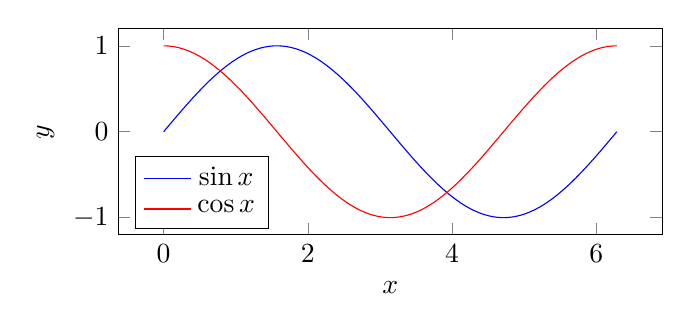
\begin{tikzpicture}
\begin{axis}[width=0.7\linewidth, height=4.2cm, xlabel={$x$},
             ylabel={$y$}, domain=0:6.283, samples=100,
             legend pos=south west]
  \addplot+[no marks] {sin(deg(x))};
  \addplot+[no marks] {cos(deg(x))};
  \legend{$\sin x$, $\cos x$}
\end{axis}
\end{tikzpicture}
\end{notefigure}
\end{demo}

\begin{tip}[Plots from Python]
Save from matplotlib with \code{plt.savefig("fig.pdf")} and include it with
\code{\includegraphics[width=0.6\linewidth]{fig.pdf}}. A PDF stays sharp at any zoom.
\end{tip}

Side by side:
\begin{demo}
\begin{notefigure}[Two images][fig:two]
  \begin{subfigure}{0.3\linewidth}\centering
    \includegraphics[width=\linewidth]{example-image-b}\caption{left}
  \end{subfigure}\quad
  \begin{subfigure}{0.3\linewidth}\centering
    \includegraphics[width=\linewidth]{example-image-c}\caption{right}
  \end{subfigure}
\end{notefigure}
\end{demo}

% =====================================================================
\section{Algorithms (pseudocode)}

\begin{demo}
\begin{algorithm}[H]
\caption{A generic iterative procedure}\label{alg:sample}
\begin{algorithmic}[1]
\Require data $D$, tolerance $\varepsilon > 0$
\State $r \gets$ initial guess
\Repeat
  \For{each item $d \in D$}
    \State update $r$ using $d$
  \EndFor
\Until{the change in $r$ is below $\varepsilon$}
\State \Return $r$
\end{algorithmic}
\end{algorithm}
\end{demo}

Always use \code{[H]} so the algorithm stays where you write it.

% =====================================================================
\section{Cross-references}

Give anything a label, then refer to it with \code{\cref}: it adds the right word
(\emph{Theorem}, \emph{Table}, \dots) and makes it a link. Use \code{\Cref} at the
start of a sentence.

\begin{demo}
By \cref{thm:sum} and \cref{def:inc}, see \cref{eq:sample},
\cref{tab:sample}, \cref{fig:plot} and \cref{alg:sample}.
\end{demo}

\begin{datatable}[Label prefixes (a habit, not a rule)][tab:prefixes]{ll}
\thead{Prefix} & \thead{For} \\
\midrule
\code{def:} \code{thm:} \code{ex:} & boxes \\
\code{eq:} & equations \\
\code{tab:} \code{fig:} \code{alg:} & tables, figures, algorithms \\
\code{sec:} & sections
\end{datatable}

\begin{important}
References show \textbf{??} until the document has been compiled twice.
\code{latexmk}, Overleaf and LaTeX Workshop do this for you.
\end{important}

% =====================================================================
\section{Slides (Beamer)}

All boxes, callouts, code blocks, tables, figures and macros work on slides as
well. Start from \code{slides.tex}; its preamble is:

\begin{demosource}
% !TEX program = xelatex
\documentclass[aspectratio=169, 9pt, t, notheorems]{beamer}
\usetheme{mynotes}               % options: see the table below
\title[Short title]{Full Title}  % [short title] appears in the footer
\subtitle{Optional subtitle}
\author{Author Name}
\website{https://example.com}    % the author name links here
\institute{Department Name, University Name}
\date{\today}

\begin{document}
\titleframe                      % title slide
\begin{frame}{Frame title}{Optional subtitle}
  ...
\end{frame}
\closingframe                    % "Thank you!" slide
\end{document}
\end{demosource}

\begin{widetable}[What is specific to slides][tab:slides]{lL}
\thead{Item} & \thead{How} \\
\midrule
Class options    & \code{aspectratio=169} (use \code{43} for 4:3), \code{9pt} (or \code{10pt}, \code{11pt}), \code{t} (top-aligned) and \code{notheorems} (required, so the template's boxes replace Beamer's). \\
Title slide      & \code{\titleframe}: no header or footer. \\
Last slide       & \code{\closingframe}: ``Thank you!'' and ``Questions \& Discussion''. Change the text with \code{\closingframe[second line][first line]}. \\
Navigation bar   & At the top: every \code{\section} name, with one dot per slide. Hide it with \code{\usetheme[nonavigation]{mynotes}}. \\
Section slides   & Off by default. \code{\usetheme[sectionframes]{mynotes}} adds one at every \code{\section}; or write \code{\sectionframe} by hand. \\
Footer           & Author (linked to \code{\website}) \textbar\ short title \textbar\ slide number. \\
Compact boxes    & On slides, box titles are run in (``\textbf{Theorem 2.1.} If\dots'') and the padding is smaller, to fit more per slide. \\
Code             & A frame containing \code{python}, \code{codeblock} or \code{terminal} needs \code{\begin{frame}[fragile]}. \\
Step by step     & \code{\pause} between items, or \code{\item<2->} to show an item from the second step on. \\
Two columns      & \code{\begin{columns}[T]} with \code{\begin{column}{0.48\textwidth}}. \\
Emphasis         & \code{\alert{...}} (red) and \code{\hl{...}} (highlighter). \\
Beamer blocks    & \code{block}, \code{alertblock}, \code{exampleblock} are restyled to match.
\end{widetable}

% =====================================================================
\section{Customization}

\subsection{Package and theme options}

\begin{datatable}[Options][tab:options]{ll}
\thead{Option} & \thead{Effect} \\
\midrule
\code{classicmath} & Latin Modern for all math (notes and slides) \\
\code{sectionframes} & A section slide at every \code{\section} (slides) \\
\code{nonavigation} & No navigation bar at the top (slides) \\
\code{\showsolutionsfalse} & Hide all solutions (preamble command)
\end{datatable}

\subsection{Colors}

Redefine any template color in your preamble, after \code{\usepackage{mynotes}}
or \code{\usetheme{mynotes}}:

\begin{demosource}
\definecolor{accent}{RGB}{120,40,140}   % headings, links, slide titles
\definecolor{thmframe}{RGB}{0,90,60}    % theorem box: bar
\definecolor{thmback}{RGB}{232,245,239} % theorem box: background
\end{demosource}

\begin{widetable}[Color names][tab:colors]{LL}
\thead{Name} & \thead{Used for} \\
\midrule
\code{accent}, \code{bodytext} & Headings, links and slide titles; body text \\
\code{defframe}, \code{defback} & Definitions \\
\code{exframe}, \code{exback} & Examples \\
\code{thmframe}, \code{thmback} & Theorems, lemmas, propositions, corollaries \\
\code{exerframe}, \code{exerback} & Exercises \\
\code{remframe}, \code{remback} & Remarks \\
\code{co-blue}, \code{co-cyan}, \code{co-green}, \code{co-orange}, \code{co-red}, \code{co-gray} & Callouts and plot lines \\
\code{hlcolor}, \code{codebg}, \code{tablehead}, \code{tablestripe} & Highlighter, code background, table header and stripes
\end{widetable}

\subsection{Fonts and page layout}

Fonts are set at the top of \code{mynotes-core.sty} with \code{fontspec}; the page
size and margins of the notes are set at the top of \code{mynotes.sty} with
\code{geometry}. To use US Letter paper, replace \code{a4paper} with
\code{letterpaper} there.

% =====================================================================
\section{Troubleshooting}

\begin{faq}[``Compile with XeLaTeX or LuaLaTeX, not pdfLaTeX'']
Switch the compiler: Overleaf \textbf{Menu} $\to$ \textbf{Compiler} $\to$
\textbf{XeLaTeX}; locally run \code{latexmk}, which reads \code{latexmkrc}.
\end{faq}

\begin{faq}[``The font IBMPlexMono cannot be found'']
The \code{fonts/} folder must be in the same folder as the main \code{.tex} file.
Keep the folder structure when you copy the template.
\end{faq}

\begin{faq}[References show ``??'']
Compile again; cross-references need two runs.
\end{faq}

\begin{faq}[Errors on a slide with code]
Add \code{[fragile]} to that frame: \code{\begin{frame}[fragile]{Title}}.
\end{faq}

\begin{faq}[Errors from inline code inside a heading or caption]
Use \code{\texttt{...}} in headings, captions and other command arguments.
\end{faq}

\begin{info}[License]
Template code: MIT License. IBM Plex Mono and Font Awesome Free fonts: SIL Open
Font License~1.1 (see \code{fonts/}).
\end{info}

\end{document}
